
% Default to the notebook output style

    


% Inherit from the specified cell style.




    
\documentclass[11pt]{article}

    
    
    \usepackage[T1]{fontenc}
    % Nicer default font (+ math font) than Computer Modern for most use cases
    \usepackage{mathpazo}

    % Basic figure setup, for now with no caption control since it's done
    % automatically by Pandoc (which extracts ![](path) syntax from Markdown).
    \usepackage{graphicx}
    % We will generate all images so they have a width \maxwidth. This means
    % that they will get their normal width if they fit onto the page, but
    % are scaled down if they would overflow the margins.
    \makeatletter
    \def\maxwidth{\ifdim\Gin@nat@width>\linewidth\linewidth
    \else\Gin@nat@width\fi}
    \makeatother
    \let\Oldincludegraphics\includegraphics
    % Set max figure width to be 80% of text width, for now hardcoded.
    \renewcommand{\includegraphics}[1]{\Oldincludegraphics[width=.8\maxwidth]{#1}}
    % Ensure that by default, figures have no caption (until we provide a
    % proper Figure object with a Caption API and a way to capture that
    % in the conversion process - todo).
    \usepackage{caption}
    \DeclareCaptionLabelFormat{nolabel}{}
    \captionsetup{labelformat=nolabel}

    \usepackage{adjustbox} % Used to constrain images to a maximum size 
    \usepackage{xcolor} % Allow colors to be defined
    \usepackage{enumerate} % Needed for markdown enumerations to work
    \usepackage{geometry} % Used to adjust the document margins
    \usepackage{amsmath} % Equations
    \usepackage{amssymb} % Equations
    \usepackage{textcomp} % defines textquotesingle
    % Hack from http://tex.stackexchange.com/a/47451/13684:
    \AtBeginDocument{%
        \def\PYZsq{\textquotesingle}% Upright quotes in Pygmentized code
    }
    \usepackage{upquote} % Upright quotes for verbatim code
    \usepackage{eurosym} % defines \euro
    \usepackage[mathletters]{ucs} % Extended unicode (utf-8) support
    \usepackage[utf8x]{inputenc} % Allow utf-8 characters in the tex document
    \usepackage{fancyvrb} % verbatim replacement that allows latex
    \usepackage{grffile} % extends the file name processing of package graphics 
                         % to support a larger range 
    % The hyperref package gives us a pdf with properly built
    % internal navigation ('pdf bookmarks' for the table of contents,
    % internal cross-reference links, web links for URLs, etc.)
    \usepackage{hyperref}
    \usepackage{longtable} % longtable support required by pandoc >1.10
    \usepackage{booktabs}  % table support for pandoc > 1.12.2
    \usepackage[inline]{enumitem} % IRkernel/repr support (it uses the enumerate* environment)
    \usepackage[normalem]{ulem} % ulem is needed to support strikethroughs (\sout)
                                % normalem makes italics be italics, not underlines
    

    
    
    % Colors for the hyperref package
    \definecolor{urlcolor}{rgb}{0,.145,.698}
    \definecolor{linkcolor}{rgb}{.71,0.21,0.01}
    \definecolor{citecolor}{rgb}{.12,.54,.11}

    % ANSI colors
    \definecolor{ansi-black}{HTML}{3E424D}
    \definecolor{ansi-black-intense}{HTML}{282C36}
    \definecolor{ansi-red}{HTML}{E75C58}
    \definecolor{ansi-red-intense}{HTML}{B22B31}
    \definecolor{ansi-green}{HTML}{00A250}
    \definecolor{ansi-green-intense}{HTML}{007427}
    \definecolor{ansi-yellow}{HTML}{DDB62B}
    \definecolor{ansi-yellow-intense}{HTML}{B27D12}
    \definecolor{ansi-blue}{HTML}{208FFB}
    \definecolor{ansi-blue-intense}{HTML}{0065CA}
    \definecolor{ansi-magenta}{HTML}{D160C4}
    \definecolor{ansi-magenta-intense}{HTML}{A03196}
    \definecolor{ansi-cyan}{HTML}{60C6C8}
    \definecolor{ansi-cyan-intense}{HTML}{258F8F}
    \definecolor{ansi-white}{HTML}{C5C1B4}
    \definecolor{ansi-white-intense}{HTML}{A1A6B2}

    % commands and environments needed by pandoc snippets
    % extracted from the output of `pandoc -s`
    \providecommand{\tightlist}{%
      \setlength{\itemsep}{0pt}\setlength{\parskip}{0pt}}
    \DefineVerbatimEnvironment{Highlighting}{Verbatim}{commandchars=\\\{\}}
    % Add ',fontsize=\small' for more characters per line
    \newenvironment{Shaded}{}{}
    \newcommand{\KeywordTok}[1]{\textcolor[rgb]{0.00,0.44,0.13}{\textbf{{#1}}}}
    \newcommand{\DataTypeTok}[1]{\textcolor[rgb]{0.56,0.13,0.00}{{#1}}}
    \newcommand{\DecValTok}[1]{\textcolor[rgb]{0.25,0.63,0.44}{{#1}}}
    \newcommand{\BaseNTok}[1]{\textcolor[rgb]{0.25,0.63,0.44}{{#1}}}
    \newcommand{\FloatTok}[1]{\textcolor[rgb]{0.25,0.63,0.44}{{#1}}}
    \newcommand{\CharTok}[1]{\textcolor[rgb]{0.25,0.44,0.63}{{#1}}}
    \newcommand{\StringTok}[1]{\textcolor[rgb]{0.25,0.44,0.63}{{#1}}}
    \newcommand{\CommentTok}[1]{\textcolor[rgb]{0.38,0.63,0.69}{\textit{{#1}}}}
    \newcommand{\OtherTok}[1]{\textcolor[rgb]{0.00,0.44,0.13}{{#1}}}
    \newcommand{\AlertTok}[1]{\textcolor[rgb]{1.00,0.00,0.00}{\textbf{{#1}}}}
    \newcommand{\FunctionTok}[1]{\textcolor[rgb]{0.02,0.16,0.49}{{#1}}}
    \newcommand{\RegionMarkerTok}[1]{{#1}}
    \newcommand{\ErrorTok}[1]{\textcolor[rgb]{1.00,0.00,0.00}{\textbf{{#1}}}}
    \newcommand{\NormalTok}[1]{{#1}}
    
    % Additional commands for more recent versions of Pandoc
    \newcommand{\ConstantTok}[1]{\textcolor[rgb]{0.53,0.00,0.00}{{#1}}}
    \newcommand{\SpecialCharTok}[1]{\textcolor[rgb]{0.25,0.44,0.63}{{#1}}}
    \newcommand{\VerbatimStringTok}[1]{\textcolor[rgb]{0.25,0.44,0.63}{{#1}}}
    \newcommand{\SpecialStringTok}[1]{\textcolor[rgb]{0.73,0.40,0.53}{{#1}}}
    \newcommand{\ImportTok}[1]{{#1}}
    \newcommand{\DocumentationTok}[1]{\textcolor[rgb]{0.73,0.13,0.13}{\textit{{#1}}}}
    \newcommand{\AnnotationTok}[1]{\textcolor[rgb]{0.38,0.63,0.69}{\textbf{\textit{{#1}}}}}
    \newcommand{\CommentVarTok}[1]{\textcolor[rgb]{0.38,0.63,0.69}{\textbf{\textit{{#1}}}}}
    \newcommand{\VariableTok}[1]{\textcolor[rgb]{0.10,0.09,0.49}{{#1}}}
    \newcommand{\ControlFlowTok}[1]{\textcolor[rgb]{0.00,0.44,0.13}{\textbf{{#1}}}}
    \newcommand{\OperatorTok}[1]{\textcolor[rgb]{0.40,0.40,0.40}{{#1}}}
    \newcommand{\BuiltInTok}[1]{{#1}}
    \newcommand{\ExtensionTok}[1]{{#1}}
    \newcommand{\PreprocessorTok}[1]{\textcolor[rgb]{0.74,0.48,0.00}{{#1}}}
    \newcommand{\AttributeTok}[1]{\textcolor[rgb]{0.49,0.56,0.16}{{#1}}}
    \newcommand{\InformationTok}[1]{\textcolor[rgb]{0.38,0.63,0.69}{\textbf{\textit{{#1}}}}}
    \newcommand{\WarningTok}[1]{\textcolor[rgb]{0.38,0.63,0.69}{\textbf{\textit{{#1}}}}}
    
    
    % Define a nice break command that doesn't care if a line doesn't already
    % exist.
    \def\br{\hspace*{\fill} \\* }
    % Math Jax compatability definitions
    \def\gt{>}
    \def\lt{<}
    % Document parameters
    \title{FDM\_Laplace}
    
    
    

    % Pygments definitions
    
\makeatletter
\def\PY@reset{\let\PY@it=\relax \let\PY@bf=\relax%
    \let\PY@ul=\relax \let\PY@tc=\relax%
    \let\PY@bc=\relax \let\PY@ff=\relax}
\def\PY@tok#1{\csname PY@tok@#1\endcsname}
\def\PY@toks#1+{\ifx\relax#1\empty\else%
    \PY@tok{#1}\expandafter\PY@toks\fi}
\def\PY@do#1{\PY@bc{\PY@tc{\PY@ul{%
    \PY@it{\PY@bf{\PY@ff{#1}}}}}}}
\def\PY#1#2{\PY@reset\PY@toks#1+\relax+\PY@do{#2}}

\expandafter\def\csname PY@tok@w\endcsname{\def\PY@tc##1{\textcolor[rgb]{0.73,0.73,0.73}{##1}}}
\expandafter\def\csname PY@tok@c\endcsname{\let\PY@it=\textit\def\PY@tc##1{\textcolor[rgb]{0.25,0.50,0.50}{##1}}}
\expandafter\def\csname PY@tok@cp\endcsname{\def\PY@tc##1{\textcolor[rgb]{0.74,0.48,0.00}{##1}}}
\expandafter\def\csname PY@tok@k\endcsname{\let\PY@bf=\textbf\def\PY@tc##1{\textcolor[rgb]{0.00,0.50,0.00}{##1}}}
\expandafter\def\csname PY@tok@kp\endcsname{\def\PY@tc##1{\textcolor[rgb]{0.00,0.50,0.00}{##1}}}
\expandafter\def\csname PY@tok@kt\endcsname{\def\PY@tc##1{\textcolor[rgb]{0.69,0.00,0.25}{##1}}}
\expandafter\def\csname PY@tok@o\endcsname{\def\PY@tc##1{\textcolor[rgb]{0.40,0.40,0.40}{##1}}}
\expandafter\def\csname PY@tok@ow\endcsname{\let\PY@bf=\textbf\def\PY@tc##1{\textcolor[rgb]{0.67,0.13,1.00}{##1}}}
\expandafter\def\csname PY@tok@nb\endcsname{\def\PY@tc##1{\textcolor[rgb]{0.00,0.50,0.00}{##1}}}
\expandafter\def\csname PY@tok@nf\endcsname{\def\PY@tc##1{\textcolor[rgb]{0.00,0.00,1.00}{##1}}}
\expandafter\def\csname PY@tok@nc\endcsname{\let\PY@bf=\textbf\def\PY@tc##1{\textcolor[rgb]{0.00,0.00,1.00}{##1}}}
\expandafter\def\csname PY@tok@nn\endcsname{\let\PY@bf=\textbf\def\PY@tc##1{\textcolor[rgb]{0.00,0.00,1.00}{##1}}}
\expandafter\def\csname PY@tok@ne\endcsname{\let\PY@bf=\textbf\def\PY@tc##1{\textcolor[rgb]{0.82,0.25,0.23}{##1}}}
\expandafter\def\csname PY@tok@nv\endcsname{\def\PY@tc##1{\textcolor[rgb]{0.10,0.09,0.49}{##1}}}
\expandafter\def\csname PY@tok@no\endcsname{\def\PY@tc##1{\textcolor[rgb]{0.53,0.00,0.00}{##1}}}
\expandafter\def\csname PY@tok@nl\endcsname{\def\PY@tc##1{\textcolor[rgb]{0.63,0.63,0.00}{##1}}}
\expandafter\def\csname PY@tok@ni\endcsname{\let\PY@bf=\textbf\def\PY@tc##1{\textcolor[rgb]{0.60,0.60,0.60}{##1}}}
\expandafter\def\csname PY@tok@na\endcsname{\def\PY@tc##1{\textcolor[rgb]{0.49,0.56,0.16}{##1}}}
\expandafter\def\csname PY@tok@nt\endcsname{\let\PY@bf=\textbf\def\PY@tc##1{\textcolor[rgb]{0.00,0.50,0.00}{##1}}}
\expandafter\def\csname PY@tok@nd\endcsname{\def\PY@tc##1{\textcolor[rgb]{0.67,0.13,1.00}{##1}}}
\expandafter\def\csname PY@tok@s\endcsname{\def\PY@tc##1{\textcolor[rgb]{0.73,0.13,0.13}{##1}}}
\expandafter\def\csname PY@tok@sd\endcsname{\let\PY@it=\textit\def\PY@tc##1{\textcolor[rgb]{0.73,0.13,0.13}{##1}}}
\expandafter\def\csname PY@tok@si\endcsname{\let\PY@bf=\textbf\def\PY@tc##1{\textcolor[rgb]{0.73,0.40,0.53}{##1}}}
\expandafter\def\csname PY@tok@se\endcsname{\let\PY@bf=\textbf\def\PY@tc##1{\textcolor[rgb]{0.73,0.40,0.13}{##1}}}
\expandafter\def\csname PY@tok@sr\endcsname{\def\PY@tc##1{\textcolor[rgb]{0.73,0.40,0.53}{##1}}}
\expandafter\def\csname PY@tok@ss\endcsname{\def\PY@tc##1{\textcolor[rgb]{0.10,0.09,0.49}{##1}}}
\expandafter\def\csname PY@tok@sx\endcsname{\def\PY@tc##1{\textcolor[rgb]{0.00,0.50,0.00}{##1}}}
\expandafter\def\csname PY@tok@m\endcsname{\def\PY@tc##1{\textcolor[rgb]{0.40,0.40,0.40}{##1}}}
\expandafter\def\csname PY@tok@gh\endcsname{\let\PY@bf=\textbf\def\PY@tc##1{\textcolor[rgb]{0.00,0.00,0.50}{##1}}}
\expandafter\def\csname PY@tok@gu\endcsname{\let\PY@bf=\textbf\def\PY@tc##1{\textcolor[rgb]{0.50,0.00,0.50}{##1}}}
\expandafter\def\csname PY@tok@gd\endcsname{\def\PY@tc##1{\textcolor[rgb]{0.63,0.00,0.00}{##1}}}
\expandafter\def\csname PY@tok@gi\endcsname{\def\PY@tc##1{\textcolor[rgb]{0.00,0.63,0.00}{##1}}}
\expandafter\def\csname PY@tok@gr\endcsname{\def\PY@tc##1{\textcolor[rgb]{1.00,0.00,0.00}{##1}}}
\expandafter\def\csname PY@tok@ge\endcsname{\let\PY@it=\textit}
\expandafter\def\csname PY@tok@gs\endcsname{\let\PY@bf=\textbf}
\expandafter\def\csname PY@tok@gp\endcsname{\let\PY@bf=\textbf\def\PY@tc##1{\textcolor[rgb]{0.00,0.00,0.50}{##1}}}
\expandafter\def\csname PY@tok@go\endcsname{\def\PY@tc##1{\textcolor[rgb]{0.53,0.53,0.53}{##1}}}
\expandafter\def\csname PY@tok@gt\endcsname{\def\PY@tc##1{\textcolor[rgb]{0.00,0.27,0.87}{##1}}}
\expandafter\def\csname PY@tok@err\endcsname{\def\PY@bc##1{\setlength{\fboxsep}{0pt}\fcolorbox[rgb]{1.00,0.00,0.00}{1,1,1}{\strut ##1}}}
\expandafter\def\csname PY@tok@kc\endcsname{\let\PY@bf=\textbf\def\PY@tc##1{\textcolor[rgb]{0.00,0.50,0.00}{##1}}}
\expandafter\def\csname PY@tok@kd\endcsname{\let\PY@bf=\textbf\def\PY@tc##1{\textcolor[rgb]{0.00,0.50,0.00}{##1}}}
\expandafter\def\csname PY@tok@kn\endcsname{\let\PY@bf=\textbf\def\PY@tc##1{\textcolor[rgb]{0.00,0.50,0.00}{##1}}}
\expandafter\def\csname PY@tok@kr\endcsname{\let\PY@bf=\textbf\def\PY@tc##1{\textcolor[rgb]{0.00,0.50,0.00}{##1}}}
\expandafter\def\csname PY@tok@bp\endcsname{\def\PY@tc##1{\textcolor[rgb]{0.00,0.50,0.00}{##1}}}
\expandafter\def\csname PY@tok@fm\endcsname{\def\PY@tc##1{\textcolor[rgb]{0.00,0.00,1.00}{##1}}}
\expandafter\def\csname PY@tok@vc\endcsname{\def\PY@tc##1{\textcolor[rgb]{0.10,0.09,0.49}{##1}}}
\expandafter\def\csname PY@tok@vg\endcsname{\def\PY@tc##1{\textcolor[rgb]{0.10,0.09,0.49}{##1}}}
\expandafter\def\csname PY@tok@vi\endcsname{\def\PY@tc##1{\textcolor[rgb]{0.10,0.09,0.49}{##1}}}
\expandafter\def\csname PY@tok@vm\endcsname{\def\PY@tc##1{\textcolor[rgb]{0.10,0.09,0.49}{##1}}}
\expandafter\def\csname PY@tok@sa\endcsname{\def\PY@tc##1{\textcolor[rgb]{0.73,0.13,0.13}{##1}}}
\expandafter\def\csname PY@tok@sb\endcsname{\def\PY@tc##1{\textcolor[rgb]{0.73,0.13,0.13}{##1}}}
\expandafter\def\csname PY@tok@sc\endcsname{\def\PY@tc##1{\textcolor[rgb]{0.73,0.13,0.13}{##1}}}
\expandafter\def\csname PY@tok@dl\endcsname{\def\PY@tc##1{\textcolor[rgb]{0.73,0.13,0.13}{##1}}}
\expandafter\def\csname PY@tok@s2\endcsname{\def\PY@tc##1{\textcolor[rgb]{0.73,0.13,0.13}{##1}}}
\expandafter\def\csname PY@tok@sh\endcsname{\def\PY@tc##1{\textcolor[rgb]{0.73,0.13,0.13}{##1}}}
\expandafter\def\csname PY@tok@s1\endcsname{\def\PY@tc##1{\textcolor[rgb]{0.73,0.13,0.13}{##1}}}
\expandafter\def\csname PY@tok@mb\endcsname{\def\PY@tc##1{\textcolor[rgb]{0.40,0.40,0.40}{##1}}}
\expandafter\def\csname PY@tok@mf\endcsname{\def\PY@tc##1{\textcolor[rgb]{0.40,0.40,0.40}{##1}}}
\expandafter\def\csname PY@tok@mh\endcsname{\def\PY@tc##1{\textcolor[rgb]{0.40,0.40,0.40}{##1}}}
\expandafter\def\csname PY@tok@mi\endcsname{\def\PY@tc##1{\textcolor[rgb]{0.40,0.40,0.40}{##1}}}
\expandafter\def\csname PY@tok@il\endcsname{\def\PY@tc##1{\textcolor[rgb]{0.40,0.40,0.40}{##1}}}
\expandafter\def\csname PY@tok@mo\endcsname{\def\PY@tc##1{\textcolor[rgb]{0.40,0.40,0.40}{##1}}}
\expandafter\def\csname PY@tok@ch\endcsname{\let\PY@it=\textit\def\PY@tc##1{\textcolor[rgb]{0.25,0.50,0.50}{##1}}}
\expandafter\def\csname PY@tok@cm\endcsname{\let\PY@it=\textit\def\PY@tc##1{\textcolor[rgb]{0.25,0.50,0.50}{##1}}}
\expandafter\def\csname PY@tok@cpf\endcsname{\let\PY@it=\textit\def\PY@tc##1{\textcolor[rgb]{0.25,0.50,0.50}{##1}}}
\expandafter\def\csname PY@tok@c1\endcsname{\let\PY@it=\textit\def\PY@tc##1{\textcolor[rgb]{0.25,0.50,0.50}{##1}}}
\expandafter\def\csname PY@tok@cs\endcsname{\let\PY@it=\textit\def\PY@tc##1{\textcolor[rgb]{0.25,0.50,0.50}{##1}}}

\def\PYZbs{\char`\\}
\def\PYZus{\char`\_}
\def\PYZob{\char`\{}
\def\PYZcb{\char`\}}
\def\PYZca{\char`\^}
\def\PYZam{\char`\&}
\def\PYZlt{\char`\<}
\def\PYZgt{\char`\>}
\def\PYZsh{\char`\#}
\def\PYZpc{\char`\%}
\def\PYZdl{\char`\$}
\def\PYZhy{\char`\-}
\def\PYZsq{\char`\'}
\def\PYZdq{\char`\"}
\def\PYZti{\char`\~}
% for compatibility with earlier versions
\def\PYZat{@}
\def\PYZlb{[}
\def\PYZrb{]}
\makeatother


    % Exact colors from NB
    \definecolor{incolor}{rgb}{0.0, 0.0, 0.5}
    \definecolor{outcolor}{rgb}{0.545, 0.0, 0.0}



    
    % Prevent overflowing lines due to hard-to-break entities
    \sloppy 
    % Setup hyperref package
    \hypersetup{
      breaklinks=true,  % so long urls are correctly broken across lines
      colorlinks=true,
      urlcolor=urlcolor,
      linkcolor=linkcolor,
      citecolor=citecolor,
      }
    % Slightly bigger margins than the latex defaults
    
    \geometry{verbose,tmargin=1in,bmargin=1in,lmargin=1in,rmargin=1in}
    
    

    \begin{document}
    
    
    \maketitle
    
    

    
    This tutorial by Xiaozhou Li is licensed under a Creative Commons
Attribution 4.0 International License.\\
All code examples are also licensed under the
\href{http://opensource.org/licenses/MIT}{MIT license}.

    \section{Finite Difference Methods - 2D Elliptic
Problem}\label{finite-difference-methods---2d-elliptic-problem}

    \subsection{Laplace's equation}\label{laplaces-equation}

Consider the Laplace's equation given as \[
    \nabla^2 u = 0,\quad\quad (x,y) \in D,
\] where
\(\nabla^2 = \frac{\partial^2}{\partial x^2} + \frac{\partial^2}{\partial y^2}\),
and the boundary conditions are given as 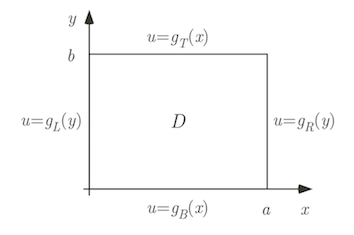
\includegraphics{img/BCs.png}

    \subsection{Finite Difference
Approximation}\label{finite-difference-approximation}

Here, we use a rectangular grid \((x_i,y_j)\), where \[
    x_i = i\Delta x, \,\,\text{for }\, i = 0,1,\ldots,N+1;\quad y_j = j\Delta y,\,\,\text{for }\, j = 0,1,\ldots,M+1.
\] Five-points scheme: \[
    -\lambda^2 u_{i+1,j} + 2(1+\lambda^2)u_{i,j} - \lambda^2u_{i-1,j} - u_{i,j+1} - u_{i,j-1} = 0,\quad\text{for}\,\, i = 1,\ldots,N,\,\, j = 1,\ldots,M,
\] where \(\lambda = \frac{\Delta y}{\Delta x}\). The boundary
conditions are -
\(x = 0: u_{0,j} = g_L(y_j), \quad\text{for }\, j = 1,\ldots,M\), -
\(x = a: u_{N+1,j} = g_R(y_j), \quad\text{for }\, j = 1,\ldots,M\), -
\(y = 0: u_{i,0} = g_B(x_i), \quad\text{for }\, i = 1,\ldots,N\), -
\(y = b: u_{i,M+1} = g_T(x_i), \quad\text{for }\, i = 1,\ldots,N\).

    \subsubsection{Building the matrix}\label{building-the-matrix}

Now, we assemble all \(N\times M\) equations into a matrix equation
\(A v = b\), where \(A\) is a \((N\times M)\times(N\times M)\) matrix
and the vector \(v\) contains the unknowns. Before assembling the matrix
\(A\), we first need to linearly order the \(u_{i,j}\) to construct this
vector. Here, we will use the common row-major ordering, which yields \[
    v = \left[u_{1,1},\ldots,u_{N,1},u_{1,2},\ldots,u_{N,2},\ldots,u_{1,M},\ldots,u_{N,M}\right]^T.
\] In general, the formula connecting \(v_\ell\) with \(u_{i,j}\) is \[
    v_\ell = u_{i,j},\quad\text{for}\,\,\ell = (j-1)N + i.
\] Then the five-points scheme becomes \[
    -\lambda^2 v_{\ell+1} + 2(1+\lambda^2)v_{\ell} - \lambda^2v_{\ell-1} - v_{\ell+N} - v_{\ell-N} = 0,\quad\text{for}\,\, \ell = 1,\ldots,N\times M,
\] which can be written in matrix form as \[
    A v = b.
\] However, at points next to a boundary one or more of the term
\(v_{\ell\pm1}\) and \(v_{\ell\pm N}\) must be modified to account for
the boundary conditions.

    \paragraph{\texorpdfstring{Assemble Matrix
\(A\)}{Assemble Matrix A}}\label{assemble-matrix-a}

For general case the matrix \(A\) (size
\((N\times M)\times(N\times M)\)) has the structure shown as follows:

\begin{equation*}
    A = \left(\begin{array}{ccccccc}T & D & & & & \\ D & T & D & & 0 & \\ & D & T & D & & \\
                                    & & \ddots & \ddots & \ddots & \\ & 0 & & D & T & D \\ 
                                    & & & & D & T\end{array}\right).
\end{equation*}

Here, the tridiagonal matrix \(T\) (size \(N \times N\))

\begin{equation*}
    T = \left(\begin{array}{ccccccc}\beta & -\lambda^2 & & & & \\ -\lambda^2 & \beta & -\lambda^2 & & 0 & \\ 
                                    & -\lambda^2 & \beta & -\lambda^2 & & \\
                                    & & \ddots & \ddots & \ddots & \\ & 0 & & -\lambda^2 & \beta & -\lambda^2 \\ 
                                    & & & & -\lambda^2 & \beta\end{array}\right),
\end{equation*}

and the diagonal matrix \(D\) (size \(N \times N\))

\begin{equation*}
    D = -I.
\end{equation*}

    \begin{Verbatim}[commandchars=\\\{\}]
{\color{incolor}In [{\color{incolor}1}]:} \PY{c+c1}{\PYZsh{}\PYZpc{}matplotlib inline}
        \PY{c+c1}{\PYZsh{}\PYZpc{}config InlineBackend.figure\PYZus{}format = \PYZsq{}retina\PYZsq{}}
        \PY{o}{\PYZpc{}}\PY{k}{matplotlib} notebook
\end{Verbatim}


    \begin{Verbatim}[commandchars=\\\{\}]
{\color{incolor}In [{\color{incolor}2}]:} \PY{c+c1}{\PYZsh{} environment setting, before any codes}
        \PY{k+kn}{import} \PY{n+nn}{numpy} \PY{k}{as} \PY{n+nn}{np}
        \PY{k+kn}{import} \PY{n+nn}{numpy}\PY{n+nn}{.}\PY{n+nn}{polynomial}\PY{n+nn}{.}\PY{n+nn}{legendre} \PY{k}{as} \PY{n+nn}{npleg}
        
        \PY{k+kn}{from} \PY{n+nn}{mpl\PYZus{}toolkits} \PY{k}{import} \PY{n}{mplot3d}
        \PY{k+kn}{from} \PY{n+nn}{mpl\PYZus{}toolkits}\PY{n+nn}{.}\PY{n+nn}{mplot3d} \PY{k}{import} \PY{n}{axes3d}
        \PY{k+kn}{import} \PY{n+nn}{matplotlib}\PY{n+nn}{.}\PY{n+nn}{pyplot} \PY{k}{as} \PY{n+nn}{plt}
        
        \PY{k+kn}{from} \PY{n+nn}{ipywidgets} \PY{k}{import} \PY{n}{interact}\PY{p}{,} \PY{n}{interactive}\PY{p}{,} \PY{n}{fixed}\PY{p}{,} \PY{n}{interact\PYZus{}manual}
        \PY{k+kn}{import} \PY{n+nn}{ipywidgets} \PY{k}{as} \PY{n+nn}{widgets}
        \PY{k+kn}{from} \PY{n+nn}{IPython}\PY{n+nn}{.}\PY{n+nn}{display} \PY{k}{import} \PY{n}{clear\PYZus{}output}\PY{p}{,} \PY{n}{display}
\end{Verbatim}


    \begin{Verbatim}[commandchars=\\\{\}]
{\color{incolor}In [{\color{incolor}3}]:} \PY{k}{def} \PY{n+nf}{generate\PYZus{}TD}\PY{p}{(}\PY{n}{N}\PY{p}{,} \PY{n}{dx}\PY{p}{,} \PY{n}{dy}\PY{p}{)}\PY{p}{:}
            \PY{n}{T} \PY{o}{=} \PY{n}{np}\PY{o}{.}\PY{n}{zeros}\PY{p}{(}\PY{p}{[}\PY{n}{N}\PY{p}{,}\PY{n}{N}\PY{p}{]}\PY{p}{)}
            \PY{n}{a} \PY{o}{=} \PY{o}{\PYZhy{}} \PY{p}{(}\PY{n}{dy}\PY{o}{/}\PY{n}{dx}\PY{p}{)}\PY{o}{*}\PY{o}{*}\PY{l+m+mi}{2}
            \PY{n}{b} \PY{o}{=} \PY{l+m+mi}{2}\PY{o}{*}\PY{p}{(}\PY{l+m+mi}{1} \PY{o}{\PYZhy{}} \PY{n}{a}\PY{p}{)}
            \PY{k}{for} \PY{n}{i} \PY{o+ow}{in} \PY{n+nb}{range}\PY{p}{(}\PY{n}{N}\PY{p}{)}\PY{p}{:}
                \PY{n}{T}\PY{p}{[}\PY{n}{i}\PY{p}{,}\PY{n}{i}\PY{p}{]} \PY{o}{+}\PY{o}{=} \PY{n}{b}
                \PY{k}{if} \PY{p}{(}\PY{n}{i} \PY{o}{\PYZlt{}} \PY{n}{N}\PY{o}{\PYZhy{}}\PY{l+m+mi}{1}\PY{p}{)}\PY{p}{:}
                    \PY{n}{T}\PY{p}{[}\PY{n}{i}\PY{p}{,}\PY{n}{i}\PY{o}{+}\PY{l+m+mi}{1}\PY{p}{]} \PY{o}{+}\PY{o}{=} \PY{n}{a}
                \PY{k}{if} \PY{p}{(}\PY{n}{i} \PY{o}{\PYZgt{}} \PY{l+m+mi}{0}\PY{p}{)}\PY{p}{:}
                    \PY{n}{T}\PY{p}{[}\PY{n}{i}\PY{p}{,}\PY{n}{i}\PY{o}{\PYZhy{}}\PY{l+m+mi}{1}\PY{p}{]} \PY{o}{+}\PY{o}{=} \PY{n}{a}
            \PY{n}{D} \PY{o}{=} \PY{o}{\PYZhy{}}\PY{n}{np}\PY{o}{.}\PY{n}{identity}\PY{p}{(}\PY{n}{N}\PY{p}{)}
            \PY{k}{return} \PY{n}{T}\PY{p}{,} \PY{n}{D}
\end{Verbatim}


    \begin{Verbatim}[commandchars=\\\{\}]
{\color{incolor}In [{\color{incolor}4}]:} \PY{k}{def} \PY{n+nf}{assemble\PYZus{}matrix\PYZus{}A}\PY{p}{(}\PY{n}{dx}\PY{p}{,} \PY{n}{dy}\PY{p}{,} \PY{n}{N}\PY{p}{,} \PY{n}{M}\PY{p}{)}\PY{p}{:}
            \PY{n}{T}\PY{p}{,} \PY{n}{D} \PY{o}{=} \PY{n}{generate\PYZus{}TD}\PY{p}{(}\PY{n}{N}\PY{p}{,} \PY{n}{dx}\PY{p}{,} \PY{n}{dy}\PY{p}{)}
            \PY{n}{A} \PY{o}{=} \PY{n}{np}\PY{o}{.}\PY{n}{zeros}\PY{p}{(}\PY{p}{[}\PY{n}{N}\PY{o}{*}\PY{n}{M}\PY{p}{,} \PY{n}{N}\PY{o}{*}\PY{n}{M}\PY{p}{]}\PY{p}{)}
            \PY{k}{for} \PY{n}{j} \PY{o+ow}{in} \PY{n+nb}{range}\PY{p}{(}\PY{n}{M}\PY{p}{)}\PY{p}{:}
                \PY{n}{A}\PY{p}{[}\PY{n}{j}\PY{o}{*}\PY{n}{N}\PY{p}{:}\PY{p}{(}\PY{n}{j}\PY{o}{+}\PY{l+m+mi}{1}\PY{p}{)}\PY{o}{*}\PY{n}{N}\PY{p}{,}\PY{n}{j}\PY{o}{*}\PY{n}{N}\PY{p}{:}\PY{p}{(}\PY{n}{j}\PY{o}{+}\PY{l+m+mi}{1}\PY{p}{)}\PY{o}{*}\PY{n}{N}\PY{p}{]} \PY{o}{+}\PY{o}{=} \PY{n}{T}
                \PY{k}{if} \PY{p}{(}\PY{n}{j} \PY{o}{\PYZlt{}} \PY{n}{M}\PY{o}{\PYZhy{}}\PY{l+m+mi}{1}\PY{p}{)}\PY{p}{:}
                    \PY{n}{A}\PY{p}{[}\PY{n}{j}\PY{o}{*}\PY{n}{N}\PY{p}{:}\PY{p}{(}\PY{n}{j}\PY{o}{+}\PY{l+m+mi}{1}\PY{p}{)}\PY{o}{*}\PY{n}{N}\PY{p}{,}\PY{p}{(}\PY{n}{j}\PY{o}{+}\PY{l+m+mi}{1}\PY{p}{)}\PY{o}{*}\PY{n}{N}\PY{p}{:}\PY{p}{(}\PY{n}{j}\PY{o}{+}\PY{l+m+mi}{2}\PY{p}{)}\PY{o}{*}\PY{n}{N}\PY{p}{]} \PY{o}{+}\PY{o}{=} \PY{n}{D}
                \PY{k}{if} \PY{p}{(}\PY{n}{j} \PY{o}{\PYZgt{}} \PY{l+m+mi}{0}\PY{p}{)}\PY{p}{:}
                    \PY{n}{A}\PY{p}{[}\PY{n}{j}\PY{o}{*}\PY{n}{N}\PY{p}{:}\PY{p}{(}\PY{n}{j}\PY{o}{+}\PY{l+m+mi}{1}\PY{p}{)}\PY{o}{*}\PY{n}{N}\PY{p}{,}\PY{p}{(}\PY{n}{j}\PY{o}{\PYZhy{}}\PY{l+m+mi}{1}\PY{p}{)}\PY{o}{*}\PY{n}{N}\PY{p}{:}\PY{n}{j}\PY{o}{*}\PY{n}{N}\PY{p}{]} \PY{o}{+}\PY{o}{=} \PY{n}{D}
            \PY{k}{return} \PY{n}{A}
        
        \PY{n}{N} \PY{o}{=} \PY{l+m+mi}{3}
        \PY{n}{M} \PY{o}{=} \PY{l+m+mi}{3}
        \PY{n}{dx} \PY{o}{=} \PY{l+m+mf}{1.}\PY{o}{/}\PY{p}{(}\PY{n}{N}\PY{o}{+}\PY{l+m+mi}{1}\PY{p}{)}
        \PY{n}{dy} \PY{o}{=} \PY{l+m+mf}{1.}\PY{o}{/}\PY{p}{(}\PY{n}{M}\PY{o}{+}\PY{l+m+mi}{1}\PY{p}{)}
        \PY{n}{T}\PY{p}{,} \PY{n}{D} \PY{o}{=} \PY{n}{generate\PYZus{}TD}\PY{p}{(}\PY{n}{N}\PY{p}{,} \PY{n}{dx}\PY{p}{,} \PY{n}{dy}\PY{p}{)}
        \PY{c+c1}{\PYZsh{}print (T)}
        \PY{n}{A} \PY{o}{=} \PY{n}{assemble\PYZus{}matrix\PYZus{}A}\PY{p}{(}\PY{n}{dx}\PY{p}{,} \PY{n}{dy}\PY{p}{,} \PY{n}{N}\PY{p}{,} \PY{n}{M}\PY{p}{)}
        \PY{c+c1}{\PYZsh{}print (A)}
        \PY{n}{plt}\PY{o}{.}\PY{n}{spy}\PY{p}{(}\PY{n}{A}\PY{p}{)}
        \PY{n}{plt}\PY{o}{.}\PY{n}{show}\PY{p}{(}\PY{p}{)}
\end{Verbatim}


    
    \begin{verbatim}
<IPython.core.display.Javascript object>
    \end{verbatim}

    
    
    \begin{verbatim}
<IPython.core.display.HTML object>
    \end{verbatim}

    
    \paragraph{\texorpdfstring{Assemble Vector
\(b\)}{Assemble Vector b}}\label{assemble-vector-b}

\begin{itemize}
\tightlist
\item
  Most components of \(b\) are zeros,
\item
  If \(v_\ell\) is next to a boundary or more, then \(b_\ell\) must be
  modified to account for the boundary condition,
\item
  In two dimension, only \(2 N\times M - 2\) components of \(b\) is
  affected by the boundary conditions.
\item
  Left boundary \(g_L\): \(b_{j N} += \lambda^2 g_L(y_j)\) for
  \(j = 0,\ldots,M-1\),
\item
  Right boundary \(g_R\): ...,
\item
  Bottom boundary \(g_B\): ...,
\item
  Top boundary \(g_T\): \(b_{(M-1)*N + i} += g_T(x_i)\) for
  \(i = 0, \ldots,N-1\).
\end{itemize}

    \begin{Verbatim}[commandchars=\\\{\}]
{\color{incolor}In [{\color{incolor}5}]:} \PY{c+c1}{\PYZsh{} Set boundary conditions}
        \PY{k}{def} \PY{n+nf}{gL}\PY{p}{(}\PY{n}{y}\PY{p}{)}\PY{p}{:}
            \PY{k}{return} \PY{l+m+mf}{0.}
        
        \PY{k}{def} \PY{n+nf}{gR}\PY{p}{(}\PY{n}{y}\PY{p}{)}\PY{p}{:}
            \PY{k}{return} \PY{l+m+mf}{0.}
        
        \PY{k}{def} \PY{n+nf}{gB}\PY{p}{(}\PY{n}{x}\PY{p}{)}\PY{p}{:}
            \PY{k}{return} \PY{l+m+mf}{0.}
        
        \PY{k}{def} \PY{n+nf}{gT}\PY{p}{(}\PY{n}{x}\PY{p}{)}\PY{p}{:}
            \PY{k}{return} \PY{l+m+mf}{1.}
            \PY{c+c1}{\PYZsh{}return x*(1\PYZhy{}x)*(4./5\PYZhy{}x)*np.exp(6*x)}
\end{Verbatim}


    \begin{Verbatim}[commandchars=\\\{\}]
{\color{incolor}In [{\color{incolor}6}]:} \PY{k}{def} \PY{n+nf}{assemble\PYZus{}vector\PYZus{}b}\PY{p}{(}\PY{n}{x}\PY{p}{,} \PY{n}{y}\PY{p}{,} \PY{n}{dx}\PY{p}{,} \PY{n}{dy}\PY{p}{,} \PY{n}{N}\PY{p}{,} \PY{n}{M}\PY{p}{,} \PY{n}{gL}\PY{p}{,} \PY{n}{gR}\PY{p}{,} \PY{n}{gB}\PY{p}{,} \PY{n}{gT}\PY{p}{)}\PY{p}{:}
            \PY{n}{b} \PY{o}{=} \PY{n}{np}\PY{o}{.}\PY{n}{zeros}\PY{p}{(}\PY{n}{N}\PY{o}{*}\PY{n}{M}\PY{p}{)}
            \PY{c+c1}{\PYZsh{} Left BCs}
            \PY{k}{for} \PY{n}{j} \PY{o+ow}{in} \PY{n+nb}{range}\PY{p}{(}\PY{n}{M}\PY{p}{)}\PY{p}{:}
                \PY{n}{b}\PY{p}{[}\PY{p}{(}\PY{n}{j}\PY{o}{\PYZhy{}}\PY{l+m+mi}{1}\PY{p}{)}\PY{o}{*}\PY{n}{N}\PY{p}{]} \PY{o}{+}\PY{o}{=} \PY{p}{(}\PY{n}{dy}\PY{o}{/}\PY{n}{dx}\PY{p}{)}\PY{o}{*}\PY{o}{*}\PY{l+m+mi}{2}\PY{o}{*}\PY{n}{gL}\PY{p}{(}\PY{n}{y}\PY{p}{[}\PY{n}{j}\PY{o}{+}\PY{l+m+mi}{1}\PY{p}{]}\PY{p}{)} 
            
            \PY{c+c1}{\PYZsh{} Right BCs}
            \PY{c+c1}{\PYZsh{} b +=}
            
            \PY{c+c1}{\PYZsh{} Bottom BCs}
            \PY{c+c1}{\PYZsh{} b +=}
            
            \PY{c+c1}{\PYZsh{} Top BCs:}
            \PY{k}{for} \PY{n}{i} \PY{o+ow}{in} \PY{n+nb}{range}\PY{p}{(}\PY{n}{N}\PY{p}{)}\PY{p}{:}
                \PY{n}{b}\PY{p}{[}\PY{p}{(}\PY{n}{M}\PY{o}{\PYZhy{}}\PY{l+m+mi}{1}\PY{p}{)}\PY{o}{*}\PY{n}{N}\PY{o}{+}\PY{n}{i}\PY{p}{]} \PY{o}{+}\PY{o}{=} \PY{n}{gT}\PY{p}{(}\PY{n}{x}\PY{p}{[}\PY{n}{i}\PY{o}{+}\PY{l+m+mi}{1}\PY{p}{]}\PY{p}{)}
            \PY{k}{return} \PY{n}{b}
\end{Verbatim}


    \begin{Verbatim}[commandchars=\\\{\}]
{\color{incolor}In [{\color{incolor}7}]:} \PY{k}{def} \PY{n+nf}{Laplace\PYZus{}solver}\PY{p}{(}\PY{n}{a}\PY{p}{,} \PY{n}{b}\PY{p}{,} \PY{n}{N}\PY{p}{,} \PY{n}{M}\PY{p}{,} \PY{n}{gL}\PY{p}{,} \PY{n}{gR}\PY{p}{,} \PY{n}{gB}\PY{p}{,} \PY{n}{gT}\PY{p}{)}\PY{p}{:}
            \PY{n}{dx} \PY{o}{=} \PY{n}{b}\PY{o}{/}\PY{p}{(}\PY{n}{M}\PY{o}{+}\PY{l+m+mi}{1}\PY{p}{)}
            \PY{n}{dy} \PY{o}{=} \PY{n}{a}\PY{o}{/}\PY{p}{(}\PY{n}{N}\PY{o}{+}\PY{l+m+mi}{1}\PY{p}{)}
            \PY{n}{x} \PY{o}{=} \PY{n}{np}\PY{o}{.}\PY{n}{linspace}\PY{p}{(}\PY{l+m+mi}{0}\PY{p}{,} \PY{n}{a}\PY{p}{,} \PY{n}{N}\PY{o}{+}\PY{l+m+mi}{2}\PY{p}{)}
            \PY{n}{y} \PY{o}{=} \PY{n}{np}\PY{o}{.}\PY{n}{linspace}\PY{p}{(}\PY{l+m+mi}{0}\PY{p}{,} \PY{n}{b}\PY{p}{,} \PY{n}{M}\PY{o}{+}\PY{l+m+mi}{2}\PY{p}{)}
            
            \PY{n}{A} \PY{o}{=} \PY{n}{assemble\PYZus{}matrix\PYZus{}A}\PY{p}{(}\PY{n}{dx}\PY{p}{,} \PY{n}{dy}\PY{p}{,} \PY{n}{N}\PY{p}{,} \PY{n}{M}\PY{p}{)}
            \PY{n}{b} \PY{o}{=} \PY{n}{assemble\PYZus{}vector\PYZus{}b}\PY{p}{(}\PY{n}{x}\PY{p}{,} \PY{n}{y}\PY{p}{,} \PY{n}{dx}\PY{p}{,} \PY{n}{dy}\PY{p}{,} \PY{n}{N}\PY{p}{,} \PY{n}{M}\PY{p}{,} \PY{n}{gL}\PY{p}{,} \PY{n}{gR}\PY{p}{,} \PY{n}{gB}\PY{p}{,} \PY{n}{gT}\PY{p}{)}
            
            \PY{n}{v} \PY{o}{=} \PY{n}{np}\PY{o}{.}\PY{n}{linalg}\PY{o}{.}\PY{n}{solve}\PY{p}{(}\PY{n}{A}\PY{p}{,}\PY{n}{b}\PY{p}{)}
            
            \PY{c+c1}{\PYZsh{} add boundary points + plotting}
            \PY{n}{u} \PY{o}{=} \PY{n}{np}\PY{o}{.}\PY{n}{zeros}\PY{p}{(}\PY{p}{[}\PY{p}{(}\PY{n}{N}\PY{o}{+}\PY{l+m+mi}{2}\PY{p}{)}\PY{p}{,}\PY{p}{(}\PY{n}{M}\PY{o}{+}\PY{l+m+mi}{2}\PY{p}{)}\PY{p}{]}\PY{p}{)}
            \PY{c+c1}{\PYZsh{}u[1:(N+1),1:(M+1)] = np.reshape(v, (N, M))}
            \PY{c+c1}{\PYZsh{} Top BCs}
            \PY{k}{for} \PY{n}{i} \PY{o+ow}{in} \PY{n+nb}{range}\PY{p}{(}\PY{n}{N}\PY{o}{+}\PY{l+m+mi}{2}\PY{p}{)}\PY{p}{:}
                \PY{n}{u}\PY{p}{[}\PY{n}{i}\PY{p}{,}\PY{n}{M}\PY{o}{+}\PY{l+m+mi}{1}\PY{p}{]} \PY{o}{=} \PY{n}{gT}\PY{p}{(}\PY{n}{x}\PY{p}{[}\PY{n}{i}\PY{p}{]}\PY{p}{)}
            \PY{n}{u} \PY{o}{=} \PY{n}{np}\PY{o}{.}\PY{n}{transpose}\PY{p}{(}\PY{n}{u}\PY{p}{)}
            \PY{n}{u}\PY{p}{[}\PY{l+m+mi}{1}\PY{p}{:}\PY{p}{(}\PY{n}{M}\PY{o}{+}\PY{l+m+mi}{1}\PY{p}{)}\PY{p}{,}\PY{l+m+mi}{1}\PY{p}{:}\PY{p}{(}\PY{n}{N}\PY{o}{+}\PY{l+m+mi}{1}\PY{p}{)}\PY{p}{]} \PY{o}{=} \PY{n}{np}\PY{o}{.}\PY{n}{reshape}\PY{p}{(}\PY{n}{v}\PY{p}{,} \PY{p}{(}\PY{n}{M}\PY{p}{,} \PY{n}{N}\PY{p}{)}\PY{p}{)}
        
            
            \PY{n}{X}\PY{p}{,} \PY{n}{Y} \PY{o}{=} \PY{n}{np}\PY{o}{.}\PY{n}{meshgrid}\PY{p}{(}\PY{n}{x}\PY{p}{,} \PY{n}{y}\PY{p}{)}
            \PY{c+c1}{\PYZsh{}Z = np.sin(2*np.pi*X)*np.sin(2*np.pi*Y)}
        
            \PY{n}{fig} \PY{o}{=} \PY{n}{plt}\PY{o}{.}\PY{n}{figure}\PY{p}{(}\PY{p}{)}
            \PY{c+c1}{\PYZsh{}ax = plt.axes(projection=\PYZsq{}3d\PYZsq{})}
            \PY{n}{ax} \PY{o}{=} \PY{n}{fig}\PY{o}{.}\PY{n}{add\PYZus{}subplot}\PY{p}{(}\PY{l+m+mi}{1}\PY{p}{,} \PY{l+m+mi}{1}\PY{p}{,} \PY{l+m+mi}{1}\PY{p}{,} \PY{n}{projection}\PY{o}{=}\PY{l+s+s1}{\PYZsq{}}\PY{l+s+s1}{3d}\PY{l+s+s1}{\PYZsq{}}\PY{p}{)}
        
            \PY{n}{ax}\PY{o}{.}\PY{n}{plot\PYZus{}surface}\PY{p}{(}\PY{n}{X}\PY{p}{,} \PY{n}{Y}\PY{p}{,} \PY{n}{u}\PY{p}{,} \PY{n}{rstride}\PY{o}{=}\PY{l+m+mi}{1}\PY{p}{,} \PY{n}{cstride}\PY{o}{=}\PY{l+m+mi}{1}\PY{p}{,}
                            \PY{n}{cmap}\PY{o}{=}\PY{l+s+s1}{\PYZsq{}}\PY{l+s+s1}{viridis}\PY{l+s+s1}{\PYZsq{}}\PY{p}{,} \PY{n}{edgecolor}\PY{o}{=}\PY{l+s+s1}{\PYZsq{}}\PY{l+s+s1}{none}\PY{l+s+s1}{\PYZsq{}}\PY{p}{)}
            \PY{n}{ax}\PY{o}{.}\PY{n}{set\PYZus{}title}\PY{p}{(}\PY{l+s+s1}{\PYZsq{}}\PY{l+s+s1}{surface}\PY{l+s+s1}{\PYZsq{}}\PY{p}{)}
            \PY{n}{plt}\PY{o}{.}\PY{n}{show}\PY{p}{(}\PY{p}{)}
            
        \PY{n}{Laplace\PYZus{}solver}\PY{p}{(}\PY{l+m+mi}{1}\PY{p}{,} \PY{l+m+mi}{1}\PY{p}{,} \PY{l+m+mi}{40}\PY{p}{,} \PY{l+m+mi}{40}\PY{p}{,} \PY{n}{gL}\PY{p}{,} \PY{n}{gR}\PY{p}{,} \PY{n}{gB}\PY{p}{,} \PY{n}{gT}\PY{p}{)}
\end{Verbatim}


    
    \begin{verbatim}
<IPython.core.display.Javascript object>
    \end{verbatim}

    
    
    \begin{verbatim}
<IPython.core.display.HTML object>
    \end{verbatim}

    
    \subsubsection{Examples}\label{examples}

\paragraph{Examples 1}\label{examples-1}

\[ 
    g_T(x) = \sin(\lambda_5 x),
\] where \(\lambda_n = \frac{n\pi}{a}\). The exaction solution is \[
    u(x,y) = \frac{\sinh(\lambda_5 y)}{\sinh(\lambda_5 b)}\sin(\lambda_5 x).
\] Here, we simply assume \(a = b = 1\)

    \begin{Verbatim}[commandchars=\\\{\}]
{\color{incolor}In [{\color{incolor}8}]:} \PY{k}{def} \PY{n+nf}{gT\PYZus{}ex1}\PY{p}{(}\PY{n}{x}\PY{p}{)}\PY{p}{:}
            \PY{k}{return} \PY{n}{np}\PY{o}{.}\PY{n}{sin}\PY{p}{(}\PY{l+m+mi}{5}\PY{o}{*}\PY{n}{np}\PY{o}{.}\PY{n}{pi}\PY{o}{*}\PY{n}{x}\PY{p}{)}
        
        \PY{k}{def} \PY{n+nf}{u\PYZus{}ex1}\PY{p}{(}\PY{n}{x}\PY{p}{,} \PY{n}{y}\PY{p}{)}\PY{p}{:}
            \PY{k}{return} \PY{n}{np}\PY{o}{.}\PY{n}{sinh}\PY{p}{(}\PY{l+m+mi}{5}\PY{o}{*}\PY{n}{np}\PY{o}{.}\PY{n}{pi}\PY{o}{*}\PY{n}{y}\PY{p}{)}\PY{o}{/}\PY{n}{np}\PY{o}{.}\PY{n}{sinh}\PY{p}{(}\PY{l+m+mi}{5}\PY{o}{*}\PY{n}{np}\PY{o}{.}\PY{n}{pi}\PY{p}{)}\PY{o}{*}\PY{n}{np}\PY{o}{.}\PY{n}{sin}\PY{p}{(}\PY{l+m+mi}{5}\PY{o}{*}\PY{n}{np}\PY{o}{.}\PY{n}{pi}\PY{o}{*}\PY{n}{x}\PY{p}{)}
        
        \PY{n}{Laplace\PYZus{}solver}\PY{p}{(}\PY{l+m+mi}{1}\PY{p}{,} \PY{l+m+mi}{1}\PY{p}{,} \PY{l+m+mi}{40}\PY{p}{,} \PY{l+m+mi}{40}\PY{p}{,} \PY{n}{gL}\PY{p}{,} \PY{n}{gR}\PY{p}{,} \PY{n}{gB}\PY{p}{,} \PY{n}{gT\PYZus{}ex1}\PY{p}{)}
\end{Verbatim}


    
    \begin{verbatim}
<IPython.core.display.Javascript object>
    \end{verbatim}

    
    
    \begin{verbatim}
<IPython.core.display.HTML object>
    \end{verbatim}

    
    \paragraph{Examples 2}\label{examples-2}

\[ 
    g_T(x) = x(1-x)(\frac{4}{5}-x)e^{6x}.
\] The fourier coefficient of exaction solution is \[
    a_n = \frac{12\lambda_n(4\gamma_n(\lambda_n^2 - 36)(\lambda_n^2+6) - 672\lambda_n^2 - 5\lambda_n^4 - 26352)}{5\sinh(\lambda_n)(\lambda_n^2 + 36)^4}
\] where \(\gamma_n = (-1)^n e^6\). Here, we simply assume \(a = b = 1\)

    \begin{Verbatim}[commandchars=\\\{\}]
{\color{incolor}In [{\color{incolor}9}]:} \PY{k}{def} \PY{n+nf}{gT\PYZus{}ex2}\PY{p}{(}\PY{n}{x}\PY{p}{)}\PY{p}{:}
            \PY{k}{return} \PY{n}{x}\PY{o}{*}\PY{p}{(}\PY{l+m+mi}{1}\PY{o}{\PYZhy{}}\PY{n}{x}\PY{p}{)}\PY{o}{*}\PY{p}{(}\PY{l+m+mf}{4.}\PY{o}{/}\PY{l+m+mi}{5}\PY{o}{\PYZhy{}}\PY{n}{x}\PY{p}{)}\PY{o}{*}\PY{n}{np}\PY{o}{.}\PY{n}{exp}\PY{p}{(}\PY{l+m+mi}{6}\PY{o}{*}\PY{n}{x}\PY{p}{)}
        
        \PY{c+c1}{\PYZsh{}def u\PYZus{}ex2(x, y):}
        \PY{c+c1}{\PYZsh{}    return np.sinh(5*np.pi*y)/np.sinh(5*np.pi)*np.sin(5*np.pi*x)}
        
        \PY{n}{Laplace\PYZus{}solver}\PY{p}{(}\PY{l+m+mi}{1}\PY{p}{,} \PY{l+m+mi}{1}\PY{p}{,} \PY{l+m+mi}{40}\PY{p}{,} \PY{l+m+mi}{40}\PY{p}{,} \PY{n}{gL}\PY{p}{,} \PY{n}{gR}\PY{p}{,} \PY{n}{gB}\PY{p}{,} \PY{n}{gT\PYZus{}ex2}\PY{p}{)}
\end{Verbatim}


    
    \begin{verbatim}
<IPython.core.display.Javascript object>
    \end{verbatim}

    
    
    \begin{verbatim}
<IPython.core.display.HTML object>
    \end{verbatim}

    
    \paragraph{Examples 3}\label{examples-3}

\[ 
    g_T(x) = \left\{\begin{array}{cl} 1 & \text{if } \frac{1}{4} \leq x \leq \frac{3}{4}, \\
                                      0 & \text{otherwise}\end{array}\right..
\] Assuming \(\frac{3}{4} < a\), the fourier coefficient of exaction
solution is given as \[
    a_n = \frac{2}{a\lambda_n\sinh(\lambda_n b)}(\cos(\lambda_n/4) - \cos(3\lambda_n/4)),
\] where \(\lambda_n = \frac{n\pi}{a}\). Here, we simply assume
\(a = b = 1\)

    \begin{Verbatim}[commandchars=\\\{\}]
{\color{incolor}In [{\color{incolor}14}]:} \PY{k}{def} \PY{n+nf}{gT\PYZus{}ex3}\PY{p}{(}\PY{n}{x}\PY{p}{)}\PY{p}{:}
             \PY{k}{if} \PY{p}{(}\PY{n}{x} \PY{o}{\PYZgt{}}\PY{o}{=} \PY{l+m+mf}{0.25} \PY{o+ow}{and} \PY{n}{x} \PY{o}{\PYZlt{}}\PY{o}{=} \PY{l+m+mf}{0.75}\PY{p}{)}\PY{p}{:}
                 \PY{k}{return} \PY{l+m+mf}{1.}
             \PY{k}{else}\PY{p}{:}
                 \PY{k}{return} \PY{l+m+mf}{0.}
         
         \PY{n}{Laplace\PYZus{}solver}\PY{p}{(}\PY{l+m+mi}{1}\PY{p}{,} \PY{l+m+mi}{1}\PY{p}{,}\PY{l+m+mi}{40}\PY{p}{,} \PY{l+m+mi}{40}\PY{p}{,} \PY{n}{gL}\PY{p}{,} \PY{n}{gR}\PY{p}{,} \PY{n}{gB}\PY{p}{,} \PY{n}{gT\PYZus{}ex3}\PY{p}{)}
\end{Verbatim}


    
    \begin{verbatim}
<IPython.core.display.Javascript object>
    \end{verbatim}

    
    
    \begin{verbatim}
<IPython.core.display.HTML object>
    \end{verbatim}

    
    \subsubsection{How to Exam the Errors?}\label{how-to-exam-the-errors}

    \begin{Verbatim}[commandchars=\\\{\}]
{\color{incolor}In [{\color{incolor}11}]:} \PY{k}{def} \PY{n+nf}{gT\PYZus{}ex4}\PY{p}{(}\PY{n}{x}\PY{p}{)}\PY{p}{:}
             \PY{k}{return} \PY{n}{np}\PY{o}{.}\PY{n}{sin}\PY{p}{(}\PY{l+m+mi}{5}\PY{o}{*}\PY{n}{np}\PY{o}{.}\PY{n}{pi}\PY{o}{*}\PY{n}{x}\PY{p}{)}
         
         \PY{k}{def} \PY{n+nf}{u\PYZus{}ex4}\PY{p}{(}\PY{n}{x}\PY{p}{,} \PY{n}{y}\PY{p}{)}\PY{p}{:}
             \PY{k}{return} \PY{n}{np}\PY{o}{.}\PY{n}{sinh}\PY{p}{(}\PY{l+m+mi}{5}\PY{o}{*}\PY{n}{np}\PY{o}{.}\PY{n}{pi}\PY{o}{*}\PY{n}{y}\PY{p}{)}\PY{o}{/}\PY{n}{np}\PY{o}{.}\PY{n}{sinh}\PY{p}{(}\PY{l+m+mi}{5}\PY{o}{*}\PY{n}{np}\PY{o}{.}\PY{n}{pi}\PY{p}{)}\PY{o}{*}\PY{n}{np}\PY{o}{.}\PY{n}{sin}\PY{p}{(}\PY{l+m+mi}{5}\PY{o}{*}\PY{n}{np}\PY{o}{.}\PY{n}{pi}\PY{o}{*}\PY{n}{x}\PY{p}{)}
         
         \PY{k}{def} \PY{n+nf}{Laplace\PYZus{}error}\PY{p}{(}\PY{n}{a}\PY{p}{,} \PY{n}{b}\PY{p}{,} \PY{n}{N}\PY{p}{,} \PY{n}{M}\PY{p}{,} \PY{n}{gL}\PY{p}{,} \PY{n}{gR}\PY{p}{,} \PY{n}{gB}\PY{p}{,} \PY{n}{gT}\PY{p}{,} \PY{n}{u\PYZus{}exact}\PY{p}{)}\PY{p}{:}
             \PY{n}{dx} \PY{o}{=} \PY{n}{b}\PY{o}{/}\PY{p}{(}\PY{n}{M}\PY{o}{+}\PY{l+m+mi}{1}\PY{p}{)}
             \PY{n}{dy} \PY{o}{=} \PY{n}{a}\PY{o}{/}\PY{p}{(}\PY{n}{N}\PY{o}{+}\PY{l+m+mi}{1}\PY{p}{)}
             \PY{n}{x} \PY{o}{=} \PY{n}{np}\PY{o}{.}\PY{n}{linspace}\PY{p}{(}\PY{l+m+mi}{0}\PY{p}{,} \PY{n}{a}\PY{p}{,} \PY{n}{N}\PY{o}{+}\PY{l+m+mi}{2}\PY{p}{)}
             \PY{n}{y} \PY{o}{=} \PY{n}{np}\PY{o}{.}\PY{n}{linspace}\PY{p}{(}\PY{l+m+mi}{0}\PY{p}{,} \PY{n}{b}\PY{p}{,} \PY{n}{M}\PY{o}{+}\PY{l+m+mi}{2}\PY{p}{)}
             
             \PY{n}{A} \PY{o}{=} \PY{n}{assemble\PYZus{}matrix\PYZus{}A}\PY{p}{(}\PY{n}{dx}\PY{p}{,} \PY{n}{dy}\PY{p}{,} \PY{n}{N}\PY{p}{,} \PY{n}{M}\PY{p}{)}
             \PY{n}{b} \PY{o}{=} \PY{n}{assemble\PYZus{}vector\PYZus{}b}\PY{p}{(}\PY{n}{x}\PY{p}{,} \PY{n}{y}\PY{p}{,} \PY{n}{dx}\PY{p}{,} \PY{n}{dy}\PY{p}{,} \PY{n}{N}\PY{p}{,} \PY{n}{M}\PY{p}{,} \PY{n}{gL}\PY{p}{,} \PY{n}{gR}\PY{p}{,} \PY{n}{gB}\PY{p}{,} \PY{n}{gT}\PY{p}{)}
             
             \PY{n}{v} \PY{o}{=} \PY{n}{np}\PY{o}{.}\PY{n}{linalg}\PY{o}{.}\PY{n}{solve}\PY{p}{(}\PY{n}{A}\PY{p}{,}\PY{n}{b}\PY{p}{)}
             
             \PY{n}{erri} \PY{o}{=} \PY{l+m+mf}{0.}
             \PY{n}{err} \PY{o}{=} \PY{n}{np}\PY{o}{.}\PY{n}{zeros}\PY{p}{(}\PY{p}{[}\PY{n}{N}\PY{p}{,}\PY{n}{M}\PY{p}{]}\PY{p}{)}
             \PY{k}{for} \PY{n}{i} \PY{o+ow}{in} \PY{n+nb}{range}\PY{p}{(}\PY{n}{N}\PY{p}{)}\PY{p}{:}
                 \PY{k}{for} \PY{n}{j} \PY{o+ow}{in} \PY{n+nb}{range}\PY{p}{(}\PY{n}{M}\PY{p}{)}\PY{p}{:}
                     \PY{n}{err}\PY{p}{[}\PY{n}{i}\PY{p}{,}\PY{n}{j}\PY{p}{]} \PY{o}{=} \PY{n}{np}\PY{o}{.}\PY{n}{abs}\PY{p}{(}\PY{n}{u\PYZus{}exact}\PY{p}{(}\PY{n}{x}\PY{p}{[}\PY{n}{i}\PY{o}{+}\PY{l+m+mi}{1}\PY{p}{]}\PY{p}{,}\PY{n}{y}\PY{p}{[}\PY{n}{j}\PY{o}{+}\PY{l+m+mi}{1}\PY{p}{]}\PY{p}{)} \PY{o}{\PYZhy{}} \PY{n}{v}\PY{p}{[}\PY{n}{j}\PY{o}{*}\PY{n}{N}\PY{o}{+}\PY{n}{i}\PY{p}{]}\PY{p}{)}
                     \PY{n}{erri} \PY{o}{=} \PY{n+nb}{max}\PY{p}{(}\PY{n}{err}\PY{p}{[}\PY{n}{i}\PY{p}{,}\PY{n}{j}\PY{p}{]}\PY{p}{,} \PY{n}{erri}\PY{p}{)}    
             \PY{k}{return} \PY{n}{erri}
             
         \PY{k}{def} \PY{n+nf}{Order\PYZus{}Verify}\PY{p}{(}\PY{n}{num}\PY{p}{,} \PY{n}{a}\PY{p}{,} \PY{n}{b}\PY{p}{,} \PY{n}{N0}\PY{p}{,} \PY{n}{M0}\PY{p}{,} \PY{n}{gL}\PY{p}{,} \PY{n}{gR}\PY{p}{,} \PY{n}{gB}\PY{p}{,} \PY{n}{gT}\PY{p}{,} \PY{n}{u\PYZus{}exact}\PY{p}{)}\PY{p}{:}
             \PY{n}{erri} \PY{o}{=} \PY{n}{np}\PY{o}{.}\PY{n}{zeros}\PY{p}{(}\PY{n}{num}\PY{p}{)}
             
             \PY{k}{for} \PY{n}{i} \PY{o+ow}{in} \PY{n+nb}{range}\PY{p}{(}\PY{n}{num}\PY{p}{)}\PY{p}{:}
                 \PY{n}{erri}\PY{p}{[}\PY{n}{i}\PY{p}{]} \PY{o}{=} \PY{n}{Laplace\PYZus{}error}\PY{p}{(}\PY{n}{a}\PY{p}{,} \PY{n}{b}\PY{p}{,} \PY{n}{N0}\PY{o}{*}\PY{l+m+mi}{2}\PY{o}{*}\PY{o}{*}\PY{n}{i}\PY{p}{,} \PY{n}{M0}\PY{o}{*}\PY{l+m+mi}{2}\PY{o}{*}\PY{o}{*}\PY{n}{i}\PY{p}{,} \PY{n}{gL}\PY{p}{,} \PY{n}{gR}\PY{p}{,} \PY{n}{gB}\PY{p}{,} \PY{n}{gT}\PY{p}{,} \PY{n}{u\PYZus{}exact}\PY{p}{)}
             
             \PY{n+nb}{print} \PY{p}{(}\PY{l+s+s2}{\PYZdq{}}\PY{l+s+s2}{ N    M  maximum error    order}\PY{l+s+s2}{\PYZdq{}}\PY{p}{)}
             \PY{k}{for} \PY{n}{i} \PY{o+ow}{in} \PY{n+nb}{range}\PY{p}{(}\PY{n}{np}\PY{o}{.}\PY{n}{size}\PY{p}{(}\PY{n}{erri}\PY{p}{)}\PY{p}{)}\PY{p}{:}
                 \PY{k}{if} \PY{p}{(}\PY{n}{i} \PY{o}{==} \PY{l+m+mi}{0}\PY{p}{)}\PY{p}{:}
                     \PY{n+nb}{print} \PY{p}{(}\PY{l+s+s2}{\PYZdq{}}\PY{l+s+si}{\PYZpc{}\PYZhy{}3d}\PY{l+s+s2}{  }\PY{l+s+si}{\PYZpc{}\PYZhy{}3d}\PY{l+s+s2}{  }\PY{l+s+si}{\PYZpc{}9.2e}\PY{l+s+s2}{        \PYZhy{}\PYZhy{}}\PY{l+s+s2}{\PYZdq{}} \PY{o}{\PYZpc{}} \PY{p}{(}\PY{n}{N0}\PY{p}{,} \PY{n}{M0}\PY{p}{,} \PY{n}{erri}\PY{p}{[}\PY{n}{i}\PY{p}{]}\PY{p}{)}\PY{p}{)}
                 \PY{k}{else}\PY{p}{:}
                     \PY{n+nb}{print} \PY{p}{(}\PY{l+s+s2}{\PYZdq{}}\PY{l+s+si}{\PYZpc{}\PYZhy{}3d}\PY{l+s+s2}{  }\PY{l+s+si}{\PYZpc{}\PYZhy{}3d}\PY{l+s+s2}{  }\PY{l+s+si}{\PYZpc{}9.2e}\PY{l+s+s2}{       }\PY{l+s+si}{\PYZpc{}4.2f}\PY{l+s+s2}{\PYZdq{}} \PY{o}{\PYZpc{}} \PY{p}{(}\PY{n}{N0}\PY{o}{*}\PY{l+m+mi}{2}\PY{o}{*}\PY{o}{*}\PY{n}{i}\PY{p}{,} \PY{n}{M0}\PY{o}{*}\PY{l+m+mi}{2}\PY{o}{*}\PY{o}{*}\PY{n}{i}\PY{p}{,} \PY{n}{erri}\PY{p}{[}\PY{n}{i}\PY{p}{]}\PY{p}{,} \PY{n}{np}\PY{o}{.}\PY{n}{log}\PY{p}{(}\PY{n}{erri}\PY{p}{[}\PY{n}{i}\PY{o}{\PYZhy{}}\PY{l+m+mi}{1}\PY{p}{]}\PY{o}{/}\PY{n}{erri}\PY{p}{[}\PY{n}{i}\PY{p}{]}\PY{p}{)}\PY{o}{/}\PY{n}{np}\PY{o}{.}\PY{n}{log}\PY{p}{(}\PY{l+m+mi}{2}\PY{p}{)}\PY{p}{)}\PY{p}{)}
             
             
         \PY{n}{Order\PYZus{}Verify}\PY{p}{(}\PY{l+m+mi}{4}\PY{p}{,} \PY{l+m+mi}{1}\PY{p}{,} \PY{l+m+mi}{1}\PY{p}{,} \PY{l+m+mi}{10}\PY{p}{,} \PY{l+m+mi}{10}\PY{p}{,} \PY{n}{gL}\PY{p}{,} \PY{n}{gR}\PY{p}{,} \PY{n}{gB}\PY{p}{,} \PY{n}{gT\PYZus{}ex4}\PY{p}{,} \PY{n}{u\PYZus{}ex4}\PY{p}{)}
\end{Verbatim}


    \begin{Verbatim}[commandchars=\\\{\}]
 N    M  maximum error    order
10   10    5.18e-02        --
20   20    1.57e-02       1.72
40   40    4.40e-03       1.83
80   80    1.15e-03       1.94

    \end{Verbatim}

    \section{The Conjugate Gradient
Method}\label{the-conjugate-gradient-method}

    \begin{Verbatim}[commandchars=\\\{\}]
{\color{incolor}In [{\color{incolor}23}]:} \PY{k}{def} \PY{n+nf}{CG}\PY{p}{(}\PY{n}{A}\PY{p}{,} \PY{n}{b}\PY{p}{,} \PY{n}{x0}\PY{p}{,} \PY{n}{n}\PY{p}{)}\PY{p}{:}
             \PY{n}{r\PYZus{}new} \PY{o}{=} \PY{n}{b} \PY{o}{\PYZhy{}} \PY{n}{np}\PY{o}{.}\PY{n}{dot}\PY{p}{(}\PY{n}{A}\PY{p}{,} \PY{n}{x0}\PY{p}{)} 
             \PY{n}{r\PYZus{}old} \PY{o}{=} \PY{n}{np}\PY{o}{.}\PY{n}{copy}\PY{p}{(}\PY{n}{np}\PY{o}{.}\PY{n}{size}\PY{p}{(}\PY{n}{x0}\PY{p}{)}\PY{p}{)}
             \PY{n}{d\PYZus{}old} \PY{o}{=} \PY{n}{np}\PY{o}{.}\PY{n}{zeros}\PY{p}{(}\PY{n}{np}\PY{o}{.}\PY{n}{size}\PY{p}{(}\PY{n}{x0}\PY{p}{)}\PY{p}{)}
             \PY{n}{x} \PY{o}{=} \PY{n}{np}\PY{o}{.}\PY{n}{copy}\PY{p}{(}\PY{n}{x0}\PY{p}{)}
             \PY{k}{for} \PY{n}{k} \PY{o+ow}{in} \PY{n+nb}{range}\PY{p}{(}\PY{n}{n}\PY{p}{)}\PY{p}{:}
                 \PY{k}{if} \PY{p}{(}\PY{n}{k} \PY{o}{==} \PY{l+m+mi}{0}\PY{p}{)}\PY{p}{:}
                     \PY{n}{d\PYZus{}new} \PY{o}{=} \PY{n}{np}\PY{o}{.}\PY{n}{copy}\PY{p}{(}\PY{n}{r\PYZus{}new}\PY{p}{)}
                 \PY{k}{else}\PY{p}{:}
                     \PY{n}{beta} \PY{o}{=} \PY{n}{np}\PY{o}{.}\PY{n}{dot}\PY{p}{(}\PY{n}{r\PYZus{}new}\PY{p}{,}\PY{n}{r\PYZus{}new}\PY{p}{)}\PY{o}{/}\PY{n}{np}\PY{o}{.}\PY{n}{dot}\PY{p}{(}\PY{n}{r\PYZus{}old}\PY{p}{,}\PY{n}{r\PYZus{}old}\PY{p}{)}
                     \PY{n}{d\PYZus{}new} \PY{o}{=} \PY{n}{r\PYZus{}new} \PY{o}{+} \PY{n}{beta}\PY{o}{*}\PY{n}{d\PYZus{}old}
                 \PY{n}{Ad} \PY{o}{=} \PY{n}{np}\PY{o}{.}\PY{n}{dot}\PY{p}{(}\PY{n}{A}\PY{p}{,} \PY{n}{d\PYZus{}new}\PY{p}{)}
                 \PY{n}{alpha} \PY{o}{=} \PY{n}{np}\PY{o}{.}\PY{n}{dot}\PY{p}{(}\PY{n}{r\PYZus{}new}\PY{p}{,}\PY{n}{r\PYZus{}new}\PY{p}{)}\PY{o}{/}\PY{n}{np}\PY{o}{.}\PY{n}{dot}\PY{p}{(}\PY{n}{d\PYZus{}new}\PY{p}{,}\PY{n}{Ad}\PY{p}{)}
                 \PY{n}{x} \PY{o}{+}\PY{o}{=} \PY{n}{alpha}\PY{o}{*}\PY{n}{d\PYZus{}new}
                 \PY{n}{d\PYZus{}old} \PY{o}{=} \PY{n}{d\PYZus{}new}
                 \PY{n}{r\PYZus{}old} \PY{o}{=} \PY{n}{r\PYZus{}new}
                 \PY{n}{r\PYZus{}new} \PY{o}{=} \PY{n}{r\PYZus{}old} \PY{o}{\PYZhy{}} \PY{n}{alpha}\PY{o}{*}\PY{n}{Ad}
             \PY{k}{return} \PY{n}{x}
         
         \PY{k}{def} \PY{n+nf}{CG\PYZus{}Test}\PY{p}{(}\PY{n}{A}\PY{p}{,} \PY{n}{b}\PY{p}{,} \PY{n}{x0}\PY{p}{,} \PY{n}{x\PYZus{}exact}\PY{p}{,} \PY{n}{n}\PY{p}{)}\PY{p}{:}
             \PY{n}{r\PYZus{}new} \PY{o}{=} \PY{n}{b} \PY{o}{\PYZhy{}} \PY{n}{np}\PY{o}{.}\PY{n}{dot}\PY{p}{(}\PY{n}{A}\PY{p}{,} \PY{n}{x0}\PY{p}{)} 
             \PY{n}{r\PYZus{}old} \PY{o}{=} \PY{n}{np}\PY{o}{.}\PY{n}{copy}\PY{p}{(}\PY{n}{np}\PY{o}{.}\PY{n}{size}\PY{p}{(}\PY{n}{x0}\PY{p}{)}\PY{p}{)}
             \PY{n}{d\PYZus{}old} \PY{o}{=} \PY{n}{np}\PY{o}{.}\PY{n}{zeros}\PY{p}{(}\PY{n}{np}\PY{o}{.}\PY{n}{size}\PY{p}{(}\PY{n}{x0}\PY{p}{)}\PY{p}{)}
             \PY{n}{x} \PY{o}{=} \PY{n}{np}\PY{o}{.}\PY{n}{copy}\PY{p}{(}\PY{n}{x0}\PY{p}{)}
             \PY{n}{err\PYZus{}A} \PY{o}{=} \PY{n}{np}\PY{o}{.}\PY{n}{zeros}\PY{p}{(}\PY{n}{n}\PY{p}{)}
             \PY{n}{err2} \PY{o}{=} \PY{n}{np}\PY{o}{.}\PY{n}{zeros}\PY{p}{(}\PY{n}{n}\PY{p}{)}
             \PY{n+nb}{print} \PY{p}{(}\PY{l+s+s2}{\PYZdq{}}\PY{l+s+s2}{iteration number   A\PYZhy{}norm     2\PYZhy{}norm}\PY{l+s+s2}{\PYZdq{}}\PY{p}{)}
             \PY{k}{for} \PY{n}{k} \PY{o+ow}{in} \PY{n+nb}{range}\PY{p}{(}\PY{n}{n}\PY{p}{)}\PY{p}{:}
                 \PY{k}{if} \PY{p}{(}\PY{n}{k} \PY{o}{==} \PY{l+m+mi}{0}\PY{p}{)}\PY{p}{:}
                     \PY{n}{d\PYZus{}new} \PY{o}{=} \PY{n}{np}\PY{o}{.}\PY{n}{copy}\PY{p}{(}\PY{n}{r\PYZus{}new}\PY{p}{)}
                 \PY{k}{else}\PY{p}{:}
                     \PY{n}{beta} \PY{o}{=} \PY{n}{np}\PY{o}{.}\PY{n}{dot}\PY{p}{(}\PY{n}{r\PYZus{}new}\PY{p}{,}\PY{n}{r\PYZus{}new}\PY{p}{)}\PY{o}{/}\PY{n}{np}\PY{o}{.}\PY{n}{dot}\PY{p}{(}\PY{n}{r\PYZus{}old}\PY{p}{,}\PY{n}{r\PYZus{}old}\PY{p}{)}
                     \PY{n}{d\PYZus{}new} \PY{o}{=} \PY{n}{r\PYZus{}new} \PY{o}{+} \PY{n}{beta}\PY{o}{*}\PY{n}{d\PYZus{}old}
                 \PY{n}{Ad} \PY{o}{=} \PY{n}{np}\PY{o}{.}\PY{n}{dot}\PY{p}{(}\PY{n}{A}\PY{p}{,} \PY{n}{d\PYZus{}new}\PY{p}{)}
                 \PY{n}{alpha} \PY{o}{=} \PY{n}{np}\PY{o}{.}\PY{n}{dot}\PY{p}{(}\PY{n}{r\PYZus{}new}\PY{p}{,}\PY{n}{r\PYZus{}new}\PY{p}{)}\PY{o}{/}\PY{n}{np}\PY{o}{.}\PY{n}{dot}\PY{p}{(}\PY{n}{d\PYZus{}new}\PY{p}{,}\PY{n}{Ad}\PY{p}{)}
                 \PY{n}{x} \PY{o}{+}\PY{o}{=} \PY{n}{alpha}\PY{o}{*}\PY{n}{d\PYZus{}new}
                 \PY{n}{d\PYZus{}old} \PY{o}{=} \PY{n}{d\PYZus{}new}
                 \PY{n}{r\PYZus{}old} \PY{o}{=} \PY{n}{r\PYZus{}new}
                 \PY{n}{r\PYZus{}new} \PY{o}{=} \PY{n}{r\PYZus{}old} \PY{o}{\PYZhy{}} \PY{n}{alpha}\PY{o}{*}\PY{n}{Ad}
                 \PY{n}{err} \PY{o}{=} \PY{n}{x} \PY{o}{\PYZhy{}} \PY{n}{x\PYZus{}exact}
                 \PY{n}{err\PYZus{}A}\PY{p}{[}\PY{n}{k}\PY{p}{]} \PY{o}{=} \PY{n}{np}\PY{o}{.}\PY{n}{sqrt}\PY{p}{(}\PY{n}{np}\PY{o}{.}\PY{n}{dot}\PY{p}{(}\PY{n}{np}\PY{o}{.}\PY{n}{dot}\PY{p}{(}\PY{n}{err}\PY{p}{,} \PY{n}{A}\PY{p}{)}\PY{p}{,}\PY{n}{err}\PY{p}{)}\PY{p}{)}
                 \PY{n}{err2}\PY{p}{[}\PY{n}{k}\PY{p}{]} \PY{o}{=} \PY{n}{np}\PY{o}{.}\PY{n}{sqrt}\PY{p}{(}\PY{n}{np}\PY{o}{.}\PY{n}{dot}\PY{p}{(}\PY{n}{err}\PY{p}{,}\PY{n}{err}\PY{p}{)}\PY{p}{)}
                 \PY{n+nb}{print} \PY{p}{(}\PY{l+s+s2}{\PYZdq{}}\PY{l+s+si}{\PYZpc{}3d}\PY{l+s+s2}{th iteration  }\PY{l+s+si}{\PYZpc{}9.2e}\PY{l+s+s2}{  }\PY{l+s+si}{\PYZpc{}9.2e}\PY{l+s+s2}{\PYZdq{}} \PY{o}{\PYZpc{}} \PY{p}{(}\PY{n}{k}\PY{p}{,} \PY{n}{err\PYZus{}A}\PY{p}{[}\PY{n}{k}\PY{p}{]}\PY{p}{,} \PY{n}{err2}\PY{p}{[}\PY{n}{k}\PY{p}{]}\PY{p}{)}\PY{p}{)}
             \PY{k}{return} \PY{n}{x}\PY{p}{,} \PY{n}{err\PYZus{}A}
                 
         \PY{k}{def} \PY{n+nf}{Laplace\PYZus{}CG}\PY{p}{(}\PY{n}{a}\PY{p}{,} \PY{n}{b}\PY{p}{,} \PY{n}{N}\PY{p}{,} \PY{n}{M}\PY{p}{,} \PY{n}{gL}\PY{p}{,} \PY{n}{gR}\PY{p}{,} \PY{n}{gB}\PY{p}{,} \PY{n}{gT}\PY{p}{,} \PY{n}{u\PYZus{}exact}\PY{p}{)}\PY{p}{:}
             \PY{n}{dx} \PY{o}{=} \PY{n}{b}\PY{o}{/}\PY{p}{(}\PY{n}{M}\PY{o}{+}\PY{l+m+mi}{1}\PY{p}{)}
             \PY{n}{dy} \PY{o}{=} \PY{n}{a}\PY{o}{/}\PY{p}{(}\PY{n}{N}\PY{o}{+}\PY{l+m+mi}{1}\PY{p}{)}
             \PY{n}{x} \PY{o}{=} \PY{n}{np}\PY{o}{.}\PY{n}{linspace}\PY{p}{(}\PY{l+m+mi}{0}\PY{p}{,} \PY{n}{a}\PY{p}{,} \PY{n}{N}\PY{o}{+}\PY{l+m+mi}{2}\PY{p}{)}
             \PY{n}{y} \PY{o}{=} \PY{n}{np}\PY{o}{.}\PY{n}{linspace}\PY{p}{(}\PY{l+m+mi}{0}\PY{p}{,} \PY{n}{b}\PY{p}{,} \PY{n}{M}\PY{o}{+}\PY{l+m+mi}{2}\PY{p}{)}
             
             \PY{n}{A} \PY{o}{=} \PY{n}{assemble\PYZus{}matrix\PYZus{}A}\PY{p}{(}\PY{n}{dx}\PY{p}{,} \PY{n}{dy}\PY{p}{,} \PY{n}{N}\PY{p}{,} \PY{n}{M}\PY{p}{)}
             \PY{n}{b} \PY{o}{=} \PY{n}{assemble\PYZus{}vector\PYZus{}b}\PY{p}{(}\PY{n}{x}\PY{p}{,} \PY{n}{y}\PY{p}{,} \PY{n}{dx}\PY{p}{,} \PY{n}{dy}\PY{p}{,} \PY{n}{N}\PY{p}{,} \PY{n}{M}\PY{p}{,} \PY{n}{gL}\PY{p}{,} \PY{n}{gR}\PY{p}{,} \PY{n}{gB}\PY{p}{,} \PY{n}{gT}\PY{p}{)}
             
             \PY{c+c1}{\PYZsh{} direct method}
             \PY{n}{v} \PY{o}{=} \PY{n}{np}\PY{o}{.}\PY{n}{linalg}\PY{o}{.}\PY{n}{solve}\PY{p}{(}\PY{n}{A}\PY{p}{,}\PY{n}{b}\PY{p}{)}
             
             \PY{c+c1}{\PYZsh{} CG}
             \PY{n}{v0} \PY{o}{=} \PY{n}{np}\PY{o}{.}\PY{n}{zeros}\PY{p}{(}\PY{n}{np}\PY{o}{.}\PY{n}{size}\PY{p}{(}\PY{n}{v}\PY{p}{)}\PY{p}{)}
             \PY{c+c1}{\PYZsh{}for i in range(10):}
             \PY{c+c1}{\PYZsh{}    print (i, np.linalg.norm(v \PYZhy{} CG(A, b, v0, i)))}
             \PY{n}{v\PYZus{}CG}\PY{p}{,} \PY{n}{err\PYZus{}A} \PY{o}{=} \PY{n}{CG\PYZus{}Test}\PY{p}{(}\PY{n}{A}\PY{p}{,} \PY{n}{b}\PY{p}{,} \PY{n}{v0}\PY{p}{,} \PY{n}{v}\PY{p}{,} \PY{l+m+mi}{40}\PY{p}{)}
             \PY{c+c1}{\PYZsh{}plt.plot(range(20), err\PYZus{}A)}
             \PY{c+c1}{\PYZsh{}plt.show()}
                 
         \PY{n}{Laplace\PYZus{}CG}\PY{p}{(}\PY{l+m+mi}{1}\PY{p}{,} \PY{l+m+mi}{1}\PY{p}{,} \PY{l+m+mi}{40}\PY{p}{,} \PY{l+m+mi}{40}\PY{p}{,} \PY{n}{gL}\PY{p}{,} \PY{n}{gR}\PY{p}{,} \PY{n}{gB}\PY{p}{,} \PY{n}{gT\PYZus{}ex4}\PY{p}{,} \PY{n}{u\PYZus{}ex4}\PY{p}{)}
\end{Verbatim}


    \begin{Verbatim}[commandchars=\\\{\}]
iteration number   A-norm     2-norm
  0th iteration   2.12e+00   3.08e+00
  1th iteration   1.35e+00   2.21e+00
  2th iteration   8.99e-01   1.57e+00
  3th iteration   6.08e-01   1.10e+00
  4th iteration   4.14e-01   7.63e-01
  5th iteration   2.82e-01   5.27e-01
  6th iteration   1.93e-01   3.62e-01
  7th iteration   1.32e-01   2.49e-01
  8th iteration   9.05e-02   1.71e-01
  9th iteration   6.20e-02   1.17e-01
 10th iteration   4.25e-02   8.02e-02
 11th iteration   2.91e-02   5.49e-02
 12th iteration   1.99e-02   3.76e-02
 13th iteration   1.36e-02   2.58e-02
 14th iteration   9.34e-03   1.76e-02
 15th iteration   6.40e-03   1.21e-02
 16th iteration   4.38e-03   8.28e-03
 17th iteration   3.00e-03   5.67e-03
 18th iteration   2.06e-03   3.88e-03
 19th iteration   1.41e-03   2.66e-03
 20th iteration   9.65e-04   1.82e-03
 21th iteration   6.74e-04   1.27e-03
 22th iteration   5.43e-04   1.01e-03
 23th iteration   4.00e-04   7.55e-04
 24th iteration   2.79e-04   5.25e-04
 25th iteration   2.19e-04   4.08e-04
 26th iteration   1.66e-04   3.12e-04
 27th iteration   1.17e-04   2.19e-04
 28th iteration   9.32e-05   1.74e-04
 29th iteration   6.87e-05   1.30e-04
 30th iteration   4.96e-05   9.28e-05
 31th iteration   4.00e-05   7.50e-05
 32th iteration   2.86e-05   5.38e-05
 33th iteration   2.18e-05   4.04e-05
 34th iteration   1.69e-05   3.16e-05
 35th iteration   1.21e-05   2.24e-05
 36th iteration   9.64e-06   1.78e-05
 37th iteration   7.02e-06   1.29e-05
 38th iteration   5.25e-06   9.43e-06
 39th iteration   4.09e-06   7.28e-06

    \end{Verbatim}

    \subsection{The Preconditioned Conjugate Gradient
Method}\label{the-preconditioned-conjugate-gradient-method}


    % Add a bibliography block to the postdoc
    
    
    
    \end{document}
